\documentclass[10pt]{beamer}
% \documentclass[handout,10pt]{beamer}
\usepackage{my_style}

%%%%%%%%%%%%%%%%%%%%%%%%%%%%%%%%%%%%%%%%%%%%%%%%%%%%%%%%%%%%%%%%%%%%%%%%
\title[Math/CS 375]{Lecture 04 - A}
\subtitle{\S 3.1 Nonlinear Problems and the Bisection Method}

\begin{document}
% -------------------------------------------------
\begin{frame}
  \titlepage
\end{frame}
% -------------------------------------------------
\begin{frame}{Goals}
We will answer these questions:\\[3mm]
\begin{itemize}
    \item What makes solving nonlinear problems difficult? 
    \item What are some rudimentary strategies to find general locations of roots?
    \item How does the bisection method find a root? 
    \item How can we describe how quickly it finds the root?
\end{itemize}
\end{frame}
%%%%%%%%%%%%%%%%%%%%%%%%%%%%%%%%%%%%%%%%%%%%%%%%%%%%%%%%%%%%%%%%%%%%%%%
\sectionframe{Rootfinding}
%%%%%%%%%%%%%%%%%%%%%%%%%%%%%%%%%%%%%%%%%%%%%%%%%%%%%%%%%%%%%%%%%%%%%%%
\begin{frame}{Linear vs. Nonlinear}
\begin{itemize}
    \item We can solve a \textbf{Linear problem} $Ax=b$, e.g.
    \begin{equation}
    \begin{cases}
    \phantom{-}2x + 2y = 4 \\
    -3x + 5y = 2
    \end{cases}
    \end{equation}
    \item How about this \textbf{nonlinear problem}? 
    \begin{equation}
    \begin{cases}
    x^2 + y = 4 \\
    \cos(x) + y^2 = 2
    \end{cases}
    \end{equation}

    \question{
    \begin{itemize}
        \item Can you solve the nonlinear problem by hand?
        \item How many solutions are there?
        \item Is there even a solution? 
        \item How can we systematically approach the problem?
    \end{itemize}
    }
\end{itemize}
\end{frame}
% -------------------------------------------------

\begin{frame}{Root Finding}
\define{Root finding}{ 
    Given a function $f(x)$, the \textbf{root finding problem} seeks the number(s) $x$ such that $f(x) = 0$. The number $x$ is called the \textbf{root}.
}
\begin{center}
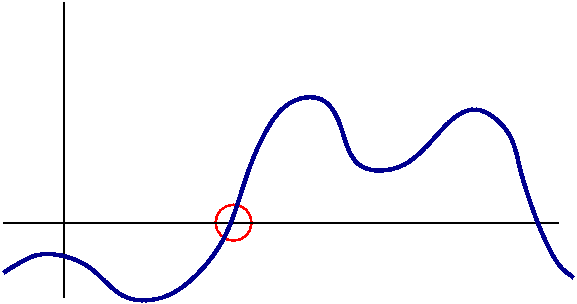
\includegraphics[scale=0.3]{figs/root.png}
\end{center}
Difficulty when $f(x)$ is nonlinear:
\begin{itemize}
    \item An analytic solution may not exist
    \item There may be multiple solutions
    \item There may be no solutions at all
\end{itemize}
\end{frame}

% -------------------------------------------------
\begin{frame}{Strategy: Iterate}

\begin{itemize}
\item For most nonlinear equations an algebraic “one‐shot” solution \textbf{does not exist}\footnote{Few exceptions: quadratics, cubics, etc.}. Consider solving the equation: 
$$\cos(x) = x$$


\item Only option is to \emph{approximate} the  root.

\begin{block}{Strategy}
Start with an initial guess $x_0$. Sequentially improve 
      \[
        x_0,\;x_1,\;x_2,\;\dots
      \]
in a way that makes $f(x_k)$ smaller and smaller. If $f(x_k)\approx0$, we are done.
\end{block}
\end{itemize}


\end{frame}

% -------------------------------------------------

\begin{frame}{Root Finding: Solving nonlinear equations}
Goals:
\begin{itemize}
  \item Systematically approximate roots to 1D functions
  \item Compare convergence properties of different methods
  \item Understand the pros and cons of each method
\end{itemize}
\bigskip 

Root-finding methods:
\begin{enumerate}
  \item Bisection Method
  \item Newton's Method
  \item Secant Method 
\end{enumerate}
\end{frame}

% -------------------------------------------------
\sectionframe{Bracketing}
% -------------------------------------------------


\begin{frame}{Plotting}

{\question{Nonlinear solvers require an initial guess $x_0$. What can we do get a decent starting point?
}}
\begin{itemize}

  \item<2-> Just plot the function
  \begin{figure}
      \centering
      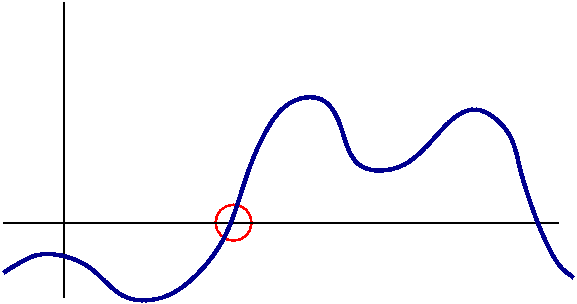
\includegraphics[width=0.3\linewidth]{figs/root.png}
  \end{figure}

  \item<2-> Look for the location where $f(x)$ crosses the $x$-axis  

  \item<2-> Works well for one-dimensional problem
    
\end{itemize}






\bigskip 
\end{frame}

% -------------------------------------------------

\begin{frame}{Plotting Example}
\begin{example}
Obtain an approximate solution $\cos{(x)} = x$ by plotting.
\end{example}
\begin{itemize}
    \item \textbf{Option 1}: Plot $\color{blue}y_1 =  x$ and $\color{mygreen}y_2 = \cos x$ and see where they intersect
    \item \textbf{Option 2}: Plot $\color{red}y = \cos x - x$ and see where it crosses the x-axis
    \begin{center}
    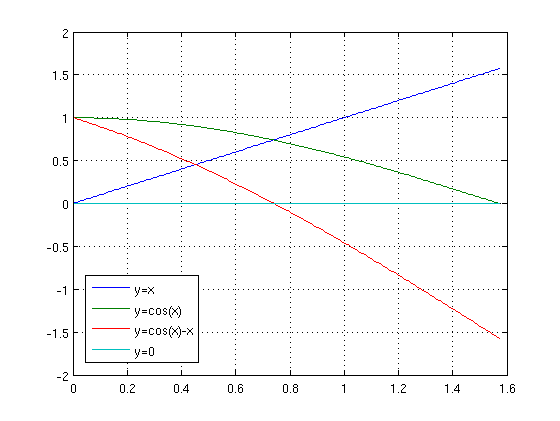
\includegraphics[scale=0.4]{figs/ch6_cosx}
    \end{center}
    \item Decent guess $x \approx 0.75$
\end{itemize}
\end{frame}

% -------------------------------------------------
%%%%%%%%%%%%%%%%%%%%%%%%%%%%%%%%%%%%%%%%%%%
\begin{frame}{Intermediate Value Theorem}

\begin{block}{Intermediate Value Theorem}
Suppose $f(x)$ is continuous on $[a,b]$. If
\[
f(a) < s < f(b)
\]
then there exists at least one point $c\in(a,b)$ such that
\[
f(c)=s.
\]
\end{block}

\vfill
\begin{block}{Let $s=0$}
Suppose $f(x)$ is continuous on $[a,b]$. If
\[
f(a) < 0 < f(b) \implies (f\text{ changes from negative to positive})
\]
then there exists at least one point $c\in(a,b)$ such that
\[
f(c)=0 \implies (f\text{ root lives somewhere inside }(a,b))
\]
\end{block}




\end{frame}

\begin{frame}{Bracket}

\define{Bracket}{
\begin{itemize}
\item A root $x$ is \textbf{bracketed} on $[a,b]$ if $f(a)$ and $f(b)$ have opposite sign
\item We call $[a,b]$ a \textbf{bracket} for the root.
\end{itemize}
}
\begin{itemize}
\item Bracketing only works when $f(x)$ is continuous
\end{itemize}
\begin{center}
\pgfimage[height=4cm]{figs/ch6_bracket}
\end{center}
\keyidea{If $f$ changes signs from $a$ to $b$, then a root must exist in between.}
\end{frame}
% -------------------------------------------------
\begin{frame}[fragile]{Bracket Algorithm}

\textbf{Steps:}\\
\begin{enumerate}
  \item Subdivide the interval into $n$ chunks.
  \item Check each subinterval for a sign change.
\end{enumerate}

\begin{lstlisting}[mathescape]
% Given: f(x), x_min, x_max, n
dx = (x_max - x_min) / n;
x_left = x_min;
i = 0;

while (i < n)
    i = i + 1;
    x_right = x_left + dx;
    if (f(x) changes sign on [x_left, x_right])
        save [x_left, x_right] as an interval with a root;
    end
    x_left = x_right;
end
\end{lstlisting}
\end{frame}
% -------------------------------------------------
\begin{frame}[containsverbatim]{How to Check for a Bracket}

\begin{block}{Option 1}
\begin{verbatim}
fa = myfunc(a);
fb = myfunc(b);
if (fa * fb < 0)
    % Save the bracket [a, b]
end
\end{verbatim}
\end{block}

\begin{block}{Option 2}
\begin{verbatim}
if (sign(fa) ~= sign(fb))
    % Save the bracket [a, b]
end
\end{verbatim}
\end{block}
\medskip
Why option 2 is better:
\begin{itemize}
    \item \textbf{Efficiency}: The function \texttt{sign()} only considers the sign bit
    \item \textbf{Safety}: Avoids potential underflow for small $f(a)*f(b)$
\end{itemize}

\end{frame}

% -------------------------------------------------
\begin{frame}{Bracketing Method}
\method{Bracketing}
{ $f(x)$, interval $[x_{\text{min}}, x_{\text{max}}]$, number of subintervals $n$ }
{List of intervals (brackets) containing roots.}
{Find general locations of the root without plotting.}
\vspace{5mm}

\keyidea{
\begin{itemize}
    \item For rootfinding, we need a starting point
    \item Plotting is a qualitative approach for preliminary investigation
    \item Bracketing is quantitative and also works for higher dimensions
\end{itemize}
}
\end{frame}



% ----------------------------

% \begin{frame}[fragile]{From FLOPs to f-evals: Measuring Cost}
% \begin{itemize}
%     \item We typically count \textbf{FLOPs} (floating point operations) to estimate computational cost.
% \begin{lstlisting}[mathescape]
% S = 0
% for i = 1 : n
%     S = S + v(i)*u(i) % 2 FLOPs per iteration 
% end
% \end{lstlisting}
%     \item In nonlinear solvers, the dominant cost is often the evaluation of the function \(f(x)\) (i.e., \textbf{f-evals}).
%     \item Counting f-evals provides a more relevant measure for algorithms like the bracketing method.

% \end{itemize}
% \end{frame}


% -------------------------------------------------
% \begin{frame}[fragile]{Cost}
% \begin{lstlisting}[mathescape]
% dx = (x_max - x_min) / n;
% x_left = x_min;
% i = 0;
% while (i < n)
%     i = i + 1;
%     x_right = x_left + dx;
%     fa = myfunc(x_right); % one f-evaluation 
%     fb = myfunc(x_left);  % one f-evaluation 
%     if (sign(fa) ~= sign(fb))
%         % Save the bracket [x_left, x_right]
%     end
%     x_left = x_right;
% end
% \end{lstlisting}

% \begin{itemize}
%     \item Bracketing costs $\mathcal{O}(n)$ f-evals.
% \end{itemize}
% \end{frame}

% -------------------------------------------------
\sectionframe{Bisection Method}
% -------------------------------------------------
\begin{frame}{High or Low}
\begin{block}{High or Low Game}
\begin{itemize}
    \item \textbf{Goal:} Guess my number.
    \item \textbf{Rule:} The number is an integer between 1 and 100. You guess a number, and I tell you whether your guess is too low or too high.
\end{itemize}
\end{block}
\vspace{3mm}
\onslide<2>{
Optimal play:
\begin{itemize}
    \item Start with 50.
    \item If the guess is too high, next guess should be 25.
    \item If the guess is too low, next guess should be 75.
    \item Continue by halving the search interval.
\end{itemize}
\keyidea{You are guaranteed to eliminate half of the wrong answers.}
}
\end{frame}

%%%%%%%%%%%%%%%%%%%%%%%%%%%%%%%%%%%%%%%%%%%%%%%%%%%%%%%%%%%%%%%%%%%%%%%%
\begin{frame}{Bisection Idea}
\begin{center}
    \pgfimage[height=3cm]{./figs/bisection}
\end{center}

Play the \textbf{high or low} game to find the root of $f(x)$:
\begin{itemize}
    \item Starting with bracket \([a,b]\).
    \item Cut the search interval in half. Is the root to the left or right?
    \item Choose the half interval containing the root. 
    \item Repeat.
\end{itemize}
\end{frame}


%%%%%%%%%%%%%%%%%%%%%%%%%%%%%%%%%%%%%%%%%%%%%%%%%%%%%%%%%%%%%%%%%%%%%%%%
\begin{frame}{Midpoints and Sign Test}
\begin{columns}
  \begin{column}{0.48\textwidth}
The \textbf{midpoint} of bracket \([a,b]\) is
\begin{equation*}
    x_m = \frac{a+b}{2}
\end{equation*}
Main steps:
\begin{enumerate}
    \item Compute the midpoint $x_m$.
    \item Evaluate \(f(x_m)\) and compare with \(f(a)\).
    \begin{itemize}
        \item If \(\mathrm{sign}(f(x_m)) = \mathrm{sign}(f(a))\), set \(a = x_m\).
        \item Otherwise, set \(b = x_m\).
    \end{itemize}
    \item Repeat until convergence.
\end{enumerate}
  \end{column}
  \begin{column}{0.48\textwidth}
  \pgfimage[height=6cm]{figs/Bisection_method}
  \end{column}
\end{columns}
\keyidea{
Always maintain the bracket.
}
\end{frame}
%%%%%%%%%%%%%%%%%%%%%%%%%%%%%%%%%%%%%%%%%%%%%%%%%%%%%%%%%%%%%%%%%%%%%%%%
\begin{frame}{Bisection Method}
\method{Bisection}
{ $f(x)$, bracket $[x_a, x_b]$, tolerance $\epsilon$ }
{Approximate solution to $f(x)=0$.}
{Reduce search interval by half each iteration.}
\vspace{5mm}
Why we like bracketing:
\begin{itemize}
    \item Easy to implement
    \item Predictable performance 
    \item A variant of this method can be extended to higher dimensions
\end{itemize}
\end{frame}

%%%%%%%%%%%%%%%%%%%%%%%%%%%%%%%%%%%%%%%%%%%%%%%%%%%%%%%%%%%%%%%%%%%%%%%%
\begin{frame}[fragile]{Bisection Update Procedure}
\begin{lstlisting}[mathescape, label=algo:bisection]
% user provides a and b such that sign(f(a)) != sign(f(b))
for k = 1, 2, ..., until convergence
    x_m = (a+b)/2;          % Compute the midpoint
    if (sign(f(x_m))==sign(f(a)))
        a = x_m;            % Root is in [x_m, b]
    else
        b = x_m;            % Root is in [a, x_m]
    end
end
\end{lstlisting}
\vspace{2mm}
\begin{itemize}
    \item Use \texttt{sign} to compare the sign of $f(x_m)$ and $f(a)$
    \item If they are the same, let $x_m$ be the new left end
    \item Otherwise, let $x_m$ be the the right end
\end{itemize}
\end{frame}

%%%%%%%%%%%%%%%%%%%%%%%%%%%%%%%%%%%%%%%%%%%%%%%%%%%%%%%%%%%%%%%%%%%%%%%%
\begin{frame}{Bisection Numerical Result}

Solve with bisection
\begin{equation*}
   f(x) = x - x^{1/3} - 2 = 0
\end{equation*}

Initial bracket: $f(a) = f(3) \approx -0.4422 \mbox{ and } f(b) = f(4) \approx 0.4126$

\begin{center}
  \small
  \renewcommand{\arraystretch}{1.3}
    \begin{tabular}{clllr}
     $k$ & \multicolumn{1}{c}{$a$}
         & \multicolumn{1}{c}{$b$}
         &  \multicolumn{1}{c}{$x_{mid}$}
         & \multicolumn{1}{c}{$f(x_{mid})$} \\ \hline
      0 &  3           & 4          &             &             \\
      1 &  3           & 4          & 3.5         & -0.01829449 \\
      2 &  3.5         & 4          & 3.75        &  0.19638375 \\
      3 &  3.5         & 3.75       & 3.625       &  0.08884159 \\
      4 &  3.5         & 3.625      & 3.5625      &  0.03522131 \\
      5 &  3.5         & 3.5625     & 3.53125     &  0.00845016 \\
      6 &  3.5         & 3.53125    & 3.515625    & -0.00492550 \\
      7 &  3.51625     & 3.53125    & 3.5234375   &  0.00176150 \\
      8 &  3.51625     & 3.5234375  & 3.51953125  & -0.00158221 \\
      9 &  3.51953125  & 3.5234375  & 3.52148438  &  0.00008959 \\
     10 &  3.51953125  & 3.52148438 & 3.52050781  & -0.00074632 \\
    \end{tabular}
\end{center}

\end{frame}

%%%%%%%%%%%%%%%%%%%%%%%%%%%%%%%%%%%%%%%%%%%%

\begin{frame}{Bisection by Hand}

\begin{example}
    Approximate the root of $f(x)=x^2-3x+1$ using the starting bracket $[1,5]$ with two iterations of the bisection method.
\end{example}

Start with $a=1$, and $b=5$. $f(a)= -1$ and $f(b)=11$
\begin{enumerate}
    \item Find the midpoint: $m = \frac{a+b}{2}=3$.
    \item Check the sign: $f(m)=f(3)=1>0$
    \item Choose the replacement: since $f(b)=11>0$, let $b=3$
                $$ a = 1, \quad b=3$$
    \item Find the midpoint: $m=\frac{a+b}{2}=2$.
    \item Check the sign: $f(2)=-1<0$
    \item Choose the replacement: since $f(a)=-1<0$, let $a=2$
                $$ a = 2, \quad b=3$$
    (Note: the answer is approximately $2.61803$)
\end{enumerate}
    
\end{frame}

% %%%%%%%%%%%%%%%%%%%%%%%%%%%%%%%%%%%%%%%%%%%%%%%%%%%%%%%%%%%%%%%%%%%%%%%%
% \sectionframe{When to Stop Iterating}
% %%%%%%%%%%%%%%%%%%%%%%%%%%%%%%%%%%%%%%%%%%%%%%%%%%%%%%%%%%%%%%%%%%%%%%%%

% \begin{frame}{How do you know when to stop?}
% \question{
% Suppose the exact solution is \(x_*\).
% How do we know when our approximation \(x_n\) is “good enough”?
% }
    
%     \vspace{3mm}

%     \begin{itemize}
%         \item<2-> \textbf{Naive answer}: Just stop when \(f(x_n) = 0\).
%         This may never occur, or may take a long time to achieve due to rounding\\[3mm]
%         \item<3-> \textbf{Real answer}: \textit{it depends}
    
%     \end{itemize}
% \end{frame}


% %%%%%%%%%%%%%%%%%%%%%%%%%%%%%%%%%%%%%%%%%%%%%%%%%%%%%%%%%%%%%%%%%%%%%%%%
% \begin{frame}{Common Stopping Conditions}
% \begin{enumerate}
%     \item \textbf{Iteration Limit:} Stop after \(N_{\text{max}}\) iterations.
%     \vspace{5mm}
%     \item \textbf{Absolute Error:} Stop when the error is smaller than \(\delta_x\):
%         \[
%          | x_* - x_n| < \delta_x.
%         \]

%     \item \textbf{Change in $x$:} Stop when the change in the solution is smaller than \(\delta_x\):
%     \[
%                 |x_n - x_{n-1}| < \delta_x.
%     \]

%     \item \textbf{Residue:} Stop when the residue is smaller than \(\delta_f\):
%     \[
%                 |f(x_n)| < \delta_f.
%     \]

%     \item \textbf{Change in $f$:} Stop when the change in residue is smaller than \(\delta_f\):
%     \[
%                 |f(x_n) - f(x_{n-1})| < \delta_f.
%     \]
% \end{enumerate}
% \end{frame}
% %%%%%%%%%%%%%%%%%%%%%%%%%%%%%%%%%%%%%%%%%%%%%%%%%%%%%%%%%%%%%%%%%%%%%%%%
% \begin{frame}[shrink]{Forward vs Backward Error}
% \begin{center}
% 	\pgfimage[height=3cm]{./figs/rootTolerance}
% \end{center}
% \begin{itemize}
%     \item The horizontal distance represents the \textbf{forward error}:
%     \[
%       e_n = |x_* - x_n|.
%     \]
%     \item The vertical distance corresponds to the \textbf{backward error}:
%     \[
%       r_n = |f(x_*) - f(x_n)| = |f(x_n)|.
%     \]
% \end{itemize}
% \end{frame}


% %%%%%%%%%%%%%%%%%%%%%%%%%%%%%%%%%%%%%%%%%%%%%%%%%%%%%%%%%%%%%%%%%%%%%%%%
% \begin{frame}[shrink]{Consider the Cases}
% \begin{itemize}
%     \item If \(|f'(x)|\) is small near the root, the forward error \(e_n\) can be large even when the residue \(r_n\) is small. Thus, it is more accurate to restrict \(\delta_x\).
%     \begin{center}
% 	    \pgfimage[height=3cm]{./figs/rootTolerance_dxbest}
%     \end{center}
%     \vspace{3ex}
%     \item If \(|f'(x)|\) is large near the root, the residue \(r_n\) changes rapidly. In this case, it is more accurate to restrict \(\delta_f\).
%     \begin{center}
% 	    \pgfimage[height=3cm]{./figs/rootTolerance_dfbest}
%     \end{center}
% \end{itemize}
% \end{frame}
% %%%%%%%%%%%%%%%%%%%%%%%%%%%%%%%%%%%%%%%%%%%%%%%%%%%%%%%%%%%%%%%%%%%%%%%%

% \begin{frame}{Relationship Between Criteria}
% \begin{itemize}
%   \item Consider the ratio between the changes in \(f(x)\) and \(x\):
%   \[
%      \frac{f(x_k) - f(x_{k-1})}{x_k - x_{k-1}}.
%   \]
%   \item As \(x_{k-1}\) and \(x_{k}\) converge to the exact solution \(x^*\), this ratio approaches the derivative \(f'(x^*)\).
%   \item Thus, we can expect (though this is not a formal proof) that 
%   \[
%      | f(x_{k})-f(x_{k-1}) | \approx |f'(x^*)|\, | x_k - x_{k-1} |
%   \]
%   as \(x_{k-1}\) and \(x_k\) approach \(x^*\).
% \keyidea{The derivative of $f$ at the root determines which stopping criteria to use. It is best to monitor both criteria.}
% \end{itemize}

% \end{frame}


%%%%%%%%%%%%%%%%%%%%%%%%%%%%%%%%%%%%%%%%%%%%%%%%%%%%%%%%%%%%%%%%%%%%%%%%
\sectionframe{Error Analysis}
%%%%%%%%%%%%%%%%%%%%%%%%%%%%%%%%%%%%%%%%%%%%%%%%%%%%%%%%%%%%%%%%%%%%%%%%
\begin{frame}[shrink]{Analysis of Bisection}
\begin{itemize}
    \item  Let \(\delta_n\) be the length of the \(n^{\text{th}}\) bracket:
\begin{align*}
    \delta_0 &= b - a \quad \text{(initial bracketing interval)}  \\
    \delta_1 &= \frac{1}{2}\,\delta_0 \\
    \delta_2 &= \frac{1}{2}\,\delta_1 = \frac{1}{4}\,\delta_0 \\
             &\ \vdots \\
    \delta_n &= \left( \frac{1}{2} \right)^n \delta_0 \\
\end{align*}
\item  Thus, the relative reduction in error is:
\[
    \frac{\delta_n}{\delta_0} = \left( \frac{1}{2} \right)^n = 2^{-n}
\]
\item or equivalently,
\[
    n = -\log_2 \left( \frac{\delta_n}{\delta_0} \right).
\]
\end{itemize}
\end{frame}

%%%%%%%%%%%%%%%%%%%%%%%%%%%%%%%%%%%%%%%%%%%%%%%%%%%%%%%%%%%%%%%%%%%%%%%%

\begin{frame}{Interpretation of Results}

\begin{block}{$\frac{\delta_n}{\delta_0} = \left( \frac{1}{2} \right)^n$}
    The ratio of the $n^{th}$ interval to the original interval is the $n^{th}$ power of 0.5.
\end{block}

\begin{block}{$n = -\log_2 \left( \frac{\delta_n}{\delta_0} \right)$}
    For some desired ratio $\delta_n/\delta_0$, it requires $|\log_2(ratio)|$ steps to achieve that reduction. 
\end{block}


\begin{center}
Example:
\renewcommand{\arraystretch}{1.3}
\begin{tabular}{c|c}
  \(n\) & \(\delta_n/\delta_0\) \\ \hline
   5   & \(3.1\times10^{-2}\) \\
  10   & \(9.8\times10^{-4}\) \\
  20   & \(9.5\times10^{-7}\) \\
  30   & \(9.3\times10^{-10}\) \\
  40   & \(9.1\times10^{-13}\) \\
  50   & \(8.9\times10^{-16}\)
\end{tabular}
\end{center}

\end{frame}
%%%%%%%%%%%%%%%%%%%%%%%%%%%%%%%%%%%%%%%%%%%%%%%%%%%%%%%%%%%%%%%%%%%%%%%%
\begin{frame}{Bisection Error}
\begin{itemize}
    \item At iteration \(n\) the true answer must be in the range
    $$
        a_n < x* < b_n
    $$
    so the error estimate is
    \[
        e_n = |x_* - c_n| \leq \frac{b_n - a_n}{2} = \frac{\delta_n}{2}.
    \]
    \item Recall that
    \[
        \delta_n = \left( \frac{1}{2} \right)^n \delta_0.
    \]
    \item Thus, the error after \(n\) steps is bounded by
    \[
        |x_* - c_n| \leq \left(\frac{1}{2}\right)^{n+1}\delta_0 
        = \left(\frac{1}{2}\right)^{n+1}(b - a).
    \]
\end{itemize}
\end{frame}

%%%%%%%%%%%%%%%%%%%%%%%%%%%%%%%%%%%%%%%%%%%%%%%%%%%%%%%%%%%%%%%%%%%%%%%%
\begin{frame}{Bisection Error Theorem}

\begin{theorem}
    If the bisection algorithm is applied to $f\in C([a,b])$ where $f(a)f(b)<0$, then after $n$ steps the error estimate is 
    $$ e_n < \frac{b-a}{2^{n+1}}.$$
\end{theorem}
\vspace{4mm}
\begin{itemize}
    \item No need to consider backward error 
    \item We have an error bound for the forward error
    \item The user may provide an error tolerance $\epsilon$ 
    \begin{itemize}
        \item Run bisection until $e_n \le \epsilon$
    \end{itemize}
\end{itemize}


\end{frame}
%%%%%%%%%%%%%%%%%%%%%%%%%%%%%%%%%%%%%%%%%%%%%%%%%%%%%%%%%%%%%%%%%%%%%%%%
\begin{frame}{Bisection: Example}

\begin{example}
What is least amount of bisection iterations needed to guarantee that the error is less than $\epsilon = 10^{-8}$ if the initial bracket is $a = -2$ and $b= 3$?
\end{example}

\vspace{3ex}
Begin by setting error $e_n$ less than tolerance $\epsilon $
\begin{align*}
&\phantom{\implies}\frac{b-a}{2^{n+1}}  < 10^{-8}\\
&\implies\frac{5}{2^{n+1}}  < 10^{-8} \qquad\qquad \mbox{substitute $a$, $b$}\\
&\implies{2^{-(n+1)}}  < 10^{-8}/5 \qquad\qquad \mbox{divide by 5}\\
&\implies -(n+1)  < \log_2(10^{-8}/5)) \qquad \mbox{log base 2 both sides}\\
&\implies n  > -\log_2(10^{-8}/5)) - 1\qquad \mbox{note the inequality flip}\\
&\implies n > 27.89
\end{align*}
So, want at least $n = 28$ steps for a guarantee.
\end{frame}


%%%%%%%%%%%%%%%%%%%%%%%%%%%%%%%%%%%%%%%%%%%%%%%%%%%%%%%%%%%%%%%%%%%%%%%%
\sectionframe{Convergence Rate}
%%%%%%%%%%%%%%%%%%%%%%%%%%%%%%%%%%%%%%%%%%%%%%%%%%%%%%%%%%%%%%%%%%%%%%%%
\begin{frame}{Convergence Rate}

{\define{Convergence Rate}{
Let $e_n = |x^* - x_n|$ be the error of an iterative method. The method is said to converge with rate $r$ if
    \begin{equation*}
      \lim_{n\rightarrow\infty} \frac{|e_{n+1}|}{|e_{n}|^{r}} \leq C 
    \end{equation*}
}}

\begin{block}{Special Cases:}
\begin{itemize}
  \item If $r=1$ and $C<1$, then the rate is \emph{linear}
  \item If $r=2$ and $C>0$, then the rate is \emph{quadratic}
  \item If $r=3$ and $C>0$, then the rate is \emph{cubic}
\end{itemize}
\end{block}
\end{frame}

% -------------------------------------------------
\begin{frame}{Determine Convergence Rate}
\begin{itemize}

    \item Rule of thumb: convergence rate is $r$ if
        $$\frac{(new\; error)}{(old\; error)^r} \approx C$$
    \begin{block}{Linear}
    $$ \text{If } \frac{new\; error}{old\; error}\approx C, \text{ then convergence is linear}$$
    \end{block}
    \begin{block}{Quadratic}
    $$ \text{If } \frac{(new\; error)}{(old\; error)^2}\approx C, \text{ then convergence is quadratic}$$
    \end{block}
        
\end{itemize}
    
\end{frame}
% -------------------------------------------------
\begin{frame}
\setbeamercovered{invisible}
\frametitle{Example}
\begin{example}
Find the convergence rate for each of the following sequences
\begin{enumerate}
\item $10^{-2}$, $10^{-3}$, $10^{-4}$, $10^{-5}$... \onslide<2->{(linear with $C=10^{-1}$)}
\item $10^{-2}$, $10^{-4}$, $10^{-6}$, $10^{-8}$... \onslide<2->{(linear with $C=10^{-2}$)}
\item $10^{-2}$, $10^{-4}$, $10^{-8}$, $10^{-16}$...\onslide<2->{(quadratic)}
\item $10^{-2}$, $10^{-6}$, $10^{-18}$, ... \onslide<2->{(cubic)}
\end{enumerate}
\end{example}
\vspace{6mm}
\onslide<3->{
    How fast is bisection converging?
}
\end{frame}
%%%%%%%%%%%%%%%%%%%%%%%%%%%%%%%%%%%%%%%%%%%%%%%%%%%%%%%%%%%%%%%%%%%%%%%%
\begin{frame}{Convergence rate of Bisection Algorithm}
\begin{itemize}
    \item We know the error estimate 
\[ |e_n| = |x_{*} - c_n | \le \frac{\delta_0}{2^{n+1}}  \]
\item Thus the ratio of new to old error is 
\[
\frac{|e_{n+1}|}{|e_n|} \approx \frac{\frac{\delta_0}{2^{n+2}} }{\frac{\delta_0}{2^{n+1}} } = \frac{1}{2}
\]
\end{itemize}
\onslide<2>{
\begin{block}{Convergence Rate}
Bisection method converges linearly with rate $C=1/2$.
\end{block}
}


\end{frame}

%%%%%%%%%%%%%%%%%%%%%%%%%%%%%%%%%%%%%%%%%%%%%%%%%%%%%%%%%%%%%%%%%%%%%%%%

\begin{frame}{Questions}

\begin{enumerate}
    \item What about bisection method makes it a good root-finding algorithm?\\[5mm] 
    \item Does this algorithm ever fail?\\[5mm]
    \item Is there a disadvantage to bisection method?\\[5mm] 
    \item Is it a fast algorithm? 
\end{enumerate}

\end{frame}
\end{document}
